
\section{Estimating Probability Distributions: Neural Networks as Function Approximators}

In previous sections, we explicitly defined probability density functions to describe relationships between variables. But there was an implicit assumption—\textbf{that we knew the correct probability distribution to use.} In reality, no single probability density function is optimal in a complex, ever-changing financial market.

\textbf{Therefore,} instead of manually specifying distributions, modern deep learning models learn an optimal function to approximate them. This is the fundamental idea behind neural networks: \textbf{they act as universal function estimators}, continuously adapting to dynamic environments.

\subsubsection*{How Neural Networks Estimate Functions}

A neural network can be viewed as a function \( f_\theta(X) \), parameterized by weights \( \theta \), which maps an input \( X \) to an output \( Y \):

\[
Y \approx f_\theta(X)
\]

Unlike traditional probability density functions, which require predefined assumptions about distributions, neural networks learn this function directly from data. Instead of defining a fixed mapping \( P(Y | X) \), the model refines its function through training, making it capable of handling highly complex, non-linear relationships.

\subsubsection*{Illustration: A Simple Neural Network}

\begin{center}
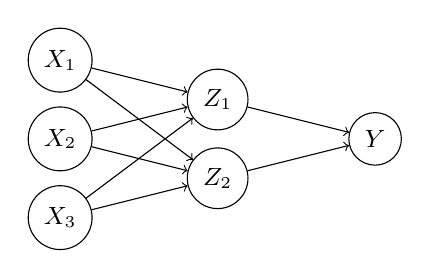
\begin{tikzpicture}[node distance=1.5cm, scale=1, every node/.style={scale=1}]
    % Input layer
    \node (x1) at (0,2) [draw, circle] {\small \(X_1\)};
    \node (x2) at (0,1) [draw, circle] {\small \(X_2\)};
    \node (x3) at (0,0) [draw, circle] {\small \(X_3\)};
    
    % Hidden layer
    \node (h1) at (2,1.5) [draw, circle] {\small \(Z_1\)};
    \node (h2) at (2,0.5) [draw, circle] {\small \(Z_2\)};
    
    % Output layer
    \node (y) at (4,1) [draw, circle] {\small \(Y\)};
    
    % Connections
    \draw[->] (x1) -- (h1);
    \draw[->] (x1) -- (h2);
    \draw[->] (x2) -- (h1);
    \draw[->] (x2) -- (h2);
    \draw[->] (x3) -- (h1);
    \draw[->] (x3) -- (h2);
    \draw[->] (h1) -- (y);
    \draw[->] (h2) -- (y);
\end{tikzpicture}
\end{center}

In this simple neural network:
\begin{itemize}
    \item \( X_1, X_2, X_3 \) are input features (e.g., trade volume, bid-ask spread, past price movement).
    \item \( Z_1, Z_2 \) are hidden neurons that extract patterns from inputs.
    \item \( Y \) is the predicted output (e.g., probability of price increasing).
\end{itemize}

\textbf{Key Idea:} Instead of explicitly defining \( P(Y | X) \), the model learns it by adjusting the weights of connections through training.

\subsubsection*{From Fixed Distributions to Adaptive Learning}

Previously, we assumed the existence of an ideal probability distribution that described our data. However, in reality:

\begin{itemize}
    \item No fixed probability density function can be truly optimal in a rapidly changing environment.
    \item Financial markets, like other dynamic systems, evolve continuously.
    \item Models must adjust to new information in real time.
\end{itemize}

\textbf{Therefore,} deep learning models estimate these functions dynamically, refining them as new data arrives. But how do we ensure that the model adapts correctly?

\subsection{Kullback-Leibler Divergence: Quantifying Information Loss in Deep Learning}

\textbf{While mutual information tells us how much two variables share, it does not tell us how much is lost when we approximate one distribution with another.} In deep learning, models do not have direct access to the true distribution of financial features—only an approximation learned through training.

\textbf{We need a way to measure how much information is lost as data propagates through layers of a neural network.}

This is precisely what the Kullback-Leibler (KL) divergence does. It quantifies how much the probability distribution of learned features in a neural network deviates from the true distribution:

\[
D_{KL}(P || Q) = \int p(x) \log \frac{p(x)}{q(x)} \, d\mu(x).
\]

where:
\begin{itemize}
    \item \( p(x) \) is the true probability distribution of a feature at a given node.
    \item \( q(x) \) is the approximated distribution learned by the neural network.
    \item \( d\mu(x) \) is the Lebesgue measure, ensuring proper integration over continuous feature spaces.
\end{itemize}

\subsubsection*{Feature Selection in Decision Trees: A Discrete Example}

Before applying KL divergence to deep learning, let’s consider a discrete case: decision trees in a financial trading model.

\paragraph{A Simple Decision Tree for Trade Execution}

Imagine an automated trading system using a decision tree to determine whether to execute a buy order based on:

\begin{itemize}
    \item Trade Volume (\textbf{High} or \textbf{Low})
    \item Price Trend (\textbf{Up} or \textbf{Down})
\end{itemize}

The tree follows this structure:

\begin{center}
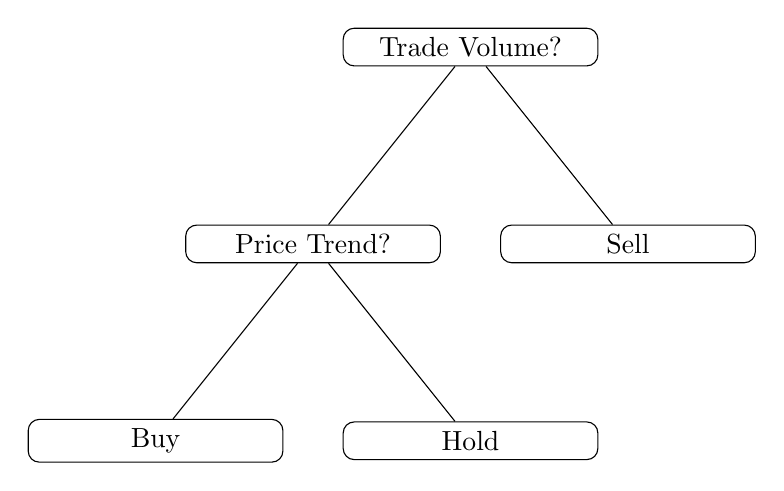
\begin{tikzpicture}[
    every node/.style={draw, rounded corners, text width=3cm, align=center},
    sibling distance=4cm,
    level distance=2.5cm
]
  % Root Node
  \node (root) {Trade Volume?}
    child { node (left) {Price Trend?}
        child { node (leftleft) {Buy} }
        child { node (leftright) {Hold} }
    }
    child { node (right) {Sell} };
\end{tikzpicture}
\end{center}

At each node, the algorithm decides whether to buy, sell, or hold. The decision-making process relies on the entropy of the dataset:

\[
\text{Information Gain} = H(Y) - H(Y | X).
\]

where:
\begin{itemize}
    \item \( H(Y) \) is the entropy of trade outcomes before the split.
    \item \( H(Y | X) \) is the entropy after splitting on a given feature.
\end{itemize}

\paragraph{From Decision Trees to Deep Neural Networks}

Decision trees work well for discrete cases but struggle with continuous and high-dimensional financial data. 

\textbf{Therefore,} deep neural networks generalize this idea by learning a feature representation at each node and refining it using KL divergence.

\subsection{Variational Information Bottleneck: KL Divergence in Deep Learning}

KL divergence is particularly crucial in variational information bottleneck (VIB) methods, where deep networks actively compress irrelevant information while preserving useful features. The VIB principle states:

\[
\max I(X; Y) - \beta D_{KL}(P(Z | X) || Q(Z)),
\]

where:
\begin{itemize}
    \item \( I(X; Y) \) is the mutual information between inputs and predictions.
    \item \( P(Z | X) \) is the learned feature distribution.
    \item \( Q(Z) \) is a constrained, low-information approximation.
    \item \( \beta \) controls how much information is discarded.
\end{itemize}

By minimizing KL divergence in a controlled way, deep networks learn to extract only the most relevant features—discarding noise while preserving signal.

---

\textbf{Takeaway:} Traditionally, we manually estimated probability density functions. Now, deep learning automates this process, continuously adapting in real time. KL divergence ensures that the model efficiently discards irrelevant data while maintaining essential structure—just like a well-optimized trading algorithm filtering out noise.



\subsection{A Concrete Example: KL Divergence in High-Frequency Trading Decisions}

To see KL divergence in action, let’s consider a high-frequency trading (HFT) system where thousands of trading machines operate independently, executing buy and sell orders in milliseconds. These machines rely on deep learning models to predict short-term price movements, but they must also filter out noise and avoid spurious correlations.

\subsubsection*{Scenario: Trading on Volume Spikes}

Imagine an HFT model that attempts to predict whether a stock price will increase in the next 10 milliseconds based on trade volume patterns. The input features for the neural network include:

\begin{itemize}
    \item \( X_1 \): Trade volume in the past 10 milliseconds.
    \item \( X_2 \): Recent bid-ask spread.
    \item \( X_3 \): Execution speed of the last 100 trades.
\end{itemize}

The model must determine whether to execute a buy order. However, trade volume alone may not be a reliable predictor—sometimes, spikes in trade volume precede price jumps, and sometimes they don’t.

\subsubsection*{Step 1: Initial Model Training}

At first, the model learns the following probability distribution:

\[
P(P | X) = P(\text{Price Increase} | X_1, X_2, X_3),
\]

which represents the likelihood that the stock price will increase given recent trading activity. However, it soon encounters a problem: 

\textbf{Not all volume spikes are created equal.} Some are genuinely predictive, while others are caused by market-wide events like algorithmic trading bursts.

\subsubsection*{Step 2: Regularizing the Model with KL Divergence}

To prevent overfitting to misleading patterns, we introduce a simplified version of the model that uses only trade volume:

\[
Q(P | X_1) = P(\text{Price Increase} | X_1),
\]

which represents a naive model that assumes price movements depend only on volume spikes. By computing the KL divergence:

\[
D_{KL}(P(P | X) || Q(P | X_1)),
\]

we measure how much information is lost when ignoring features \( X_2 \) and \( X_3 \).

\textbf{Key Observations:}
\begin{itemize}
    \item If \( D_{KL} \) is large, then bid-ask spreads and execution speed contain critical information, and removing them would degrade performance.
    \item If \( D_{KL} \) is small, then trade volume alone is sufficient, and the additional features introduce noise.
\end{itemize}

\subsubsection*{Step 3: Adaptive Trading in a Changing Market}

As the market evolves, our model continuously recalculates \( D_{KL} \) at each layer to determine which features are still useful. If the KL divergence of a feature starts decreasing over time, it means the market’s behavior has shifted, and the feature may no longer be predictive.

For instance:
\begin{itemize}
    \item If a new trading algorithm floods the market with high-frequency orders, past execution speed \( X_3 \) may lose its predictive power.
    \item If liquidity conditions change due to a macroeconomic event, bid-ask spread \( X_2 \) may become more important.
\end{itemize}

By dynamically adjusting feature selection using KL divergence, the trading model remains robust to evolving market conditions.

\subsection{The Benefit: Improved Trade Execution and Reduced Losses}

Let’s quantify the economic impact. Suppose:

\begin{itemize}
    \item Without KL divergence, the model executes 10,000 trades per day with a 52\% success rate.
    \item After applying KL divergence-based feature selection, the model eliminates noise, increasing accuracy to 54\%.
    \item Assuming an average profit of \$0.005 per share and 100 shares per trade, the difference is:
\end{itemize}

\[
(0.54 - 0.52) \times 10,000 \times 100 \times 0.005 = \mathbf{\$1,000 \text{ extra profit per day}}.
\]

Over a year, this amounts to nearly \textbf{\$250,000 in additional trading profits}, simply by improving feature selection.

\begin{quote}
\textbf{By leveraging KL divergence, our model doesn’t just trade—it adapts, evolving alongside the market to maximize efficiency and reduce unnecessary risk.}
\end{quote}

\subsection{Extracting General Patterns: How KL Divergence Shapes Learning}

The example we explored is not just a specific case—it illustrates a broader principle that applies across deep learning models. By analyzing how KL divergence refines feature selection, we can extract a general framework for how models evolve in dynamic environments like high-frequency trading.

\subsubsection*{The General Pattern: Learning as a Process of Compression and Refinement}

From our example, we can identify a recurring pattern in deep learning-based decision-making:

\begin{enumerate}
    \item \textbf{Feature Extraction:} Raw data is transformed into latent representations across multiple layers.
    \item \textbf{Regularization:} KL divergence is applied at each layer to penalize redundancy and enforce a structured representation.
    \item \textbf{Dynamic Adaptation:} The model continuously evaluates its representations, ensuring they remain relevant as the environment changes.
    \item \textbf{Causal Filtering:} KL divergence helps separate true causal influences from spurious correlations, ensuring the model learns genuine market signals.
\end{enumerate}

\subsubsection*{Why This Pattern Matters}

This structure reflects a fundamental property of intelligence: learning is an act of compression. Whether we are optimizing a trading algorithm, training a neural network, or even forming human memories, the process involves distilling essential information while discarding noise. 

\begin{itemize}
    \item \textbf{Too little compression} (\( D_{KL} \) too small): The model retains irrelevant details, overfitting to noise.
    \item \textbf{Too much compression} (\( D_{KL} \) too large): The model discards important structure, underfitting to the problem.
    \item \textbf{Balanced compression} (\( D_{KL} \) tuned correctly): The model retains only the core information necessary for accurate predictions.
\end{itemize}

\subsubsection*{Visualizing the Learning Process}

To generalize this concept, we can represent the feature refinement process with a commutative diagram. This diagram abstracts away individual equations and instead captures the relationships between layers, true feature distributions, and their regularized approximations.

\[
\begin{tikzpicture}[>=latex, scale=1.1, every node/.style={scale=1.2}]
  
  % Define matrix for the true feature distributions P(Z | X)
  \matrix (m) [matrix of math nodes, row sep=3.5em, column sep=7em] {
      X \\ 
      Z_1 \\ 
      Z_2 \\ 
      Z_3 \\ 
      P \\ % Final Prediction
  };

  % Define the simplified model Q(Z | X) to the right
  \matrix (q) [matrix of math nodes, row sep=3.5em, column sep=7em, right of=m, node distance=8cm] {
      \\  % No simplified version for X
      Q(Z_1 | X) \\ 
      Q(Z_2 | Z_1) \\ 
      Q(Z_3 | Z_2) \\ 
      Q(P | Z_3) \\ % Simplified Prediction
  };

  % Feature Transformations (Left Column)
  \path[->] (m-1-1) edge node[left] {$P(Z_1 | X)$} (m-2-1);
  \path[->] (m-2-1) edge node[left] {$P(Z_2 | Z_1)$} (m-3-1);
  \path[->] (m-3-1) edge node[left] {$P(Z_3 | Z_2)$} (m-4-1);
  \path[->] (m-4-1) edge node[left] {$P(P | Z_3)$} (m-5-1);

  % Simplified Feature Representations (Right Column)
  \path[->] (q-2-1) edge node[right] {$Q(Z_2 | Z_1)$} (q-3-1);
  \path[->] (q-3-1) edge node[right] {$Q(Z_3 | Z_2)$} (q-4-1);
  \path[->] (q-4-1) edge node[right] {$Q(P | Z_3)$} (q-5-1);

  % KL Divergence Regularization (Dashed Arrows)
  \path[->, dashed] (m-2-1.east) edge node[above] {$D_{KL}$} (q-2-1.west);
  \path[->, dashed] (m-3-1.east) edge node[above] {$D_{KL}$} (q-3-1.west);
  \path[->, dashed] (m-4-1.east) edge node[above] {$D_{KL}$} (q-4-1.west);
  \path[->, dashed] (m-5-1.east) edge node[above] {$D_{KL}(P(P | V) || Q(P | V))$} (q-5-1.west);
  
\end{tikzpicture}
\]

\subsection{Breaking Down the Commutative Diagram}

The diagram above captures the structure of learning in a deep model, where each layer refines representations and KL divergence ensures the model is only keeping the most relevant information.

\subsubsection*{Nodes and What They Represent}

\begin{itemize}
    \item \textbf{\( X \) (Raw Inputs)}: The initial data fed into the model—trade volumes, bid-ask spreads, and execution speeds.
    \item \textbf{\( Z_1, Z_2, Z_3 \) (Latent Representations)}: The abstract features extracted at increasing depths in the network. 
    \item \textbf{\( P \) (Final Prediction)}: The probability distribution over future price movements.
    \item \textbf{\( Q(Z_i | X) \) (Regularized Features)}: The simplified versions of latent features, used to prune unnecessary details.
\end{itemize}

\subsubsection*{Understanding the Arrows}

\paragraph{Solid Arrows: Transforming Features}
\begin{itemize}
    \item The vertical arrows in the left column show how the model builds complex representations:
        \[
        P(Z_1 | X), P(Z_2 | Z_1), P(Z_3 | Z_2), P(P | Z_3).
        \]
    \item The right-side vertical arrows represent the same process for a simplified version of the model, \( Q(Z | X) \), where some unnecessary features are removed.
\end{itemize}

\paragraph{Dashed Arrows: KL Divergence Regularization}
\begin{itemize}
    \item The dashed arrows indicate where KL divergence is used to penalize deviations from a minimal, compressed representation.
    \item \( D_{KL}(P(Z_i | X) || Q(Z_i | X)) \) quantifies how much information is lost when simplifying features at each layer.
\end{itemize}

\subsubsection*{Why This Matters in High-Frequency Trading}

By applying this structured learning approach, deep learning models for high-frequency trading can:
\begin{itemize}
    \item Filter out irrelevant data, preventing the model from overfitting to random noise in market fluctuations.
    \item Prioritize robust signals, ensuring that predictions rely on meaningful patterns rather than spurious correlations.
    \item Adapt to market shifts, dynamically refining which features are retained or discarded based on KL divergence measurements.
\end{itemize}

\subsection{Final Takeaway: KL Divergence as a Framework for Learning}

KL divergence is more than just a mathematical tool for deep learning—it is a guiding principle for how intelligent systems refine their understanding of the world. Whether in financial markets, artificial intelligence, or human cognition, the process follows a similar path:

\begin{itemize}
    \item Extract Features: Start with raw observations and encode them into structured representations.
    \item Apply Regularization: Use KL divergence to discard irrelevant details while preserving essential information.
    \item Adapt to Change: Continuously update the model as new information arrives, ensuring it remains aligned with reality.
\end{itemize}

\begin{quote}
\textbf{The power of KL divergence is not just in refining deep learning models—it lies in the very nature of intelligence itself.}
\end{quote}
